\newcommand{\ttt}[1]{\texttt{#1}}
\newcommand{\icc}{\texttt{icc}}
\newcommand{\gcc}{\texttt{gcc}}

\subsection{Compiler Flags and Annotations}
Compilers such as \icc{} and \gcc{} are equipped with a wide variety of command
line flags that can be used to increase the performance of the compiled code.
Similarly, the compilers understand a set of source code annotations that can
inform the compiler of certain assumptions it can make to optimize code.
Empirically, we found that that \icc{} produced the fastest code; in this
section, we present the \icc{} flags and annotations we explored.

\subsubsection{Compiler Flags}
We experimented with the following \icc{} flags.

\begin{itemize}
  \item \ttt{-xCORE-AVX2}:
    The \ttt{-x} flag informs the compiler which platform-specific
    optimizations it can use. Since we have a Xeon E5 v3 processor, we use the
    \ttt{CORE-AVX2} flag.

  \item \ttt{-fast}:
    The \ttt{-fast} flag enables entire program optimization. It's a meta-flag
    that enables a set of other flags that increase performance including
    \ttt{-O3}, \ttt{-ipo}, and \ttt{no-prec-div}.

  \item \ttt{-ansi-alias}:
    The \ttt{-ansi-alias} flag tells the compiler that our code adheres to the
    ANSI alias guidelines and allows the compiler to make aggressive
    optimizations.

  \item \ttt{-no-prec-div}:
    The \ttt{-no-prec-div} flag decreases the accuracy of floating point
    division with the benefit of increased performance. This is also enabled by
    \ttt{-fast}.

  \item \ttt{-ipo}:
    The \ttt{-ipo} flag informs the compiler to perform inter-procedural
    optimization. When \ttt{-ipo} is enabled, the compiler will optimize code
    from multiple files when they are linked together.

  \item \ttt{-prof-gen} and \ttt{-prof-use}:
    The \ttt{-prof-gen} and \ttt{-prof-use} flags allow for profile-guided
    optimization. A binary compiled with \ttt{-prof-gen} is instrumented such
    that whenever it runs, it generates a profile documenting the most
    frequently executed code paths. A binary compiled with \ttt{-prof-use} is
    built to optimize the frequently executed code paths documented in the
    profiles.
\end{itemize}

We compiled the naive matrix multiplication with all these \icc{} flags
enabled, yet the performance is negligible at best, as shown by the line titled
\ttt{compiler} in \figref{compiler}. We hypothesize that the compiler flags may
be more beneficial when used to compile less naive implementations.

\subsubsection{Compiler Annotations}
We explored two \icc{} annotations.
\begin{itemize}
  \item \ttt{restrict}:
    By default, when a function receives multiple pointers as arguments, the
    compiler must assume that the two pointers may point to overlapping regions
    of memory. This assumption can prevent the compiler from automatically
    vectorizing the code which can negatively affect performance. By annotating
    pointer arguments with \ttt{restrict}, the compiler instead assumes the
    pointers are not aliased and performs the appropriate optimizations.

  \item \ttt{aligned}:
    The alignment of data structures can affect the performance of vectorized
    instructions. Ideally, each vector of data accessed by a vector instruction
    is 16-byte aligned. The \ttt{aligned} annotation can manipulate the
    alignment of data structures to enforce alignment.
\end{itemize}

We compiled the naive matrix multiplication with all pointer arguments
annotated with \ttt{restrict}. This increased the performance of the naive
matrix multiplication to that of the Fortran implementation, as shown by the
line labelled \ttt{annotated} in \figref{compiler}. We did not yet experiment
with aligning data structures.

\begin{figure}[h]
  \centering
  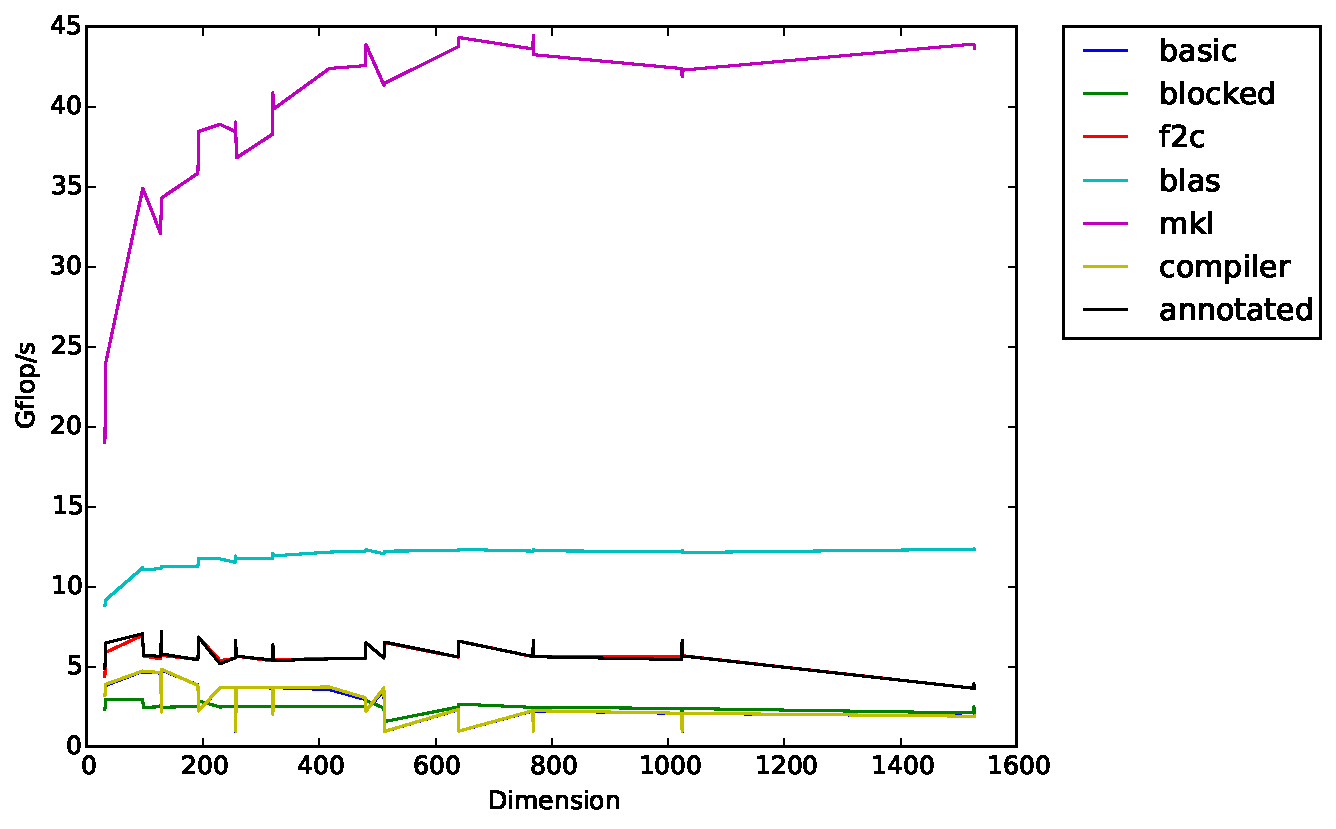
\includegraphics[width=\textwidth]{timing_compiler.pdf}
  \caption{Performance of compiler flags and annotations.}
  \label{fig:compiler}
\end{figure}
